\subsection{Critical behaviour}

\begin{frame}{Two correlation lengths}
	\begin{textblock*}{0.6\textwidth}(10mm,92mm)
		\simplephasediagram{}
	\end{textblock*}
	\begin{columns}[T]
	\column{0.5\textwidth}\centering
	Structural correlation\\
	\resizebox{\columnwidth}{!}{\begin{Large}% GNUPLOT: LaTeX picture with Postscript
\begingroup
  \makeatletter
  \providecommand\color[2][]{%
    \GenericError{(gnuplot) \space\space\space\@spaces}{%
      Package color not loaded in conjunction with
      terminal option `colourtext'%
    }{See the gnuplot documentation for explanation.%
    }{Either use 'blacktext' in gnuplot or load the package
      color.sty in LaTeX.}%
    \renewcommand\color[2][]{}%
  }%
  \providecommand\includegraphics[2][]{%
    \GenericError{(gnuplot) \space\space\space\@spaces}{%
      Package graphicx or graphics not loaded%
    }{See the gnuplot documentation for explanation.%
    }{The gnuplot epslatex terminal needs graphicx.sty or graphics.sty.}%
    \renewcommand\includegraphics[2][]{}%
  }%
  \providecommand\rotatebox[2]{#2}%
  \@ifundefined{ifGPcolor}{%
    \newif\ifGPcolor
    \GPcolortrue
  }{}%
  \@ifundefined{ifGPblacktext}{%
    \newif\ifGPblacktext
    \GPblacktexttrue
  }{}%
  % define a \g@addto@macro without @ in the name:
  \let\gplgaddtomacro\g@addto@macro
  % define empty templates for all commands taking text:
  \gdef\gplbacktext{}%
  \gdef\gplfronttext{}%
  \makeatother
  \ifGPblacktext
    % no textcolor at all
    \def\colorrgb#1{}%
    \def\colorgray#1{}%
  \else
    % gray or color?
    \ifGPcolor
      \def\colorrgb#1{\color[rgb]{#1}}%
      \def\colorgray#1{\color[gray]{#1}}%
      \expandafter\def\csname LTw\endcsname{\color{white}}%
      \expandafter\def\csname LTb\endcsname{\color{black}}%
      \expandafter\def\csname LTa\endcsname{\color{black}}%
      \expandafter\def\csname LT0\endcsname{\color[rgb]{1,0,0}}%
      \expandafter\def\csname LT1\endcsname{\color[rgb]{0,1,0}}%
      \expandafter\def\csname LT2\endcsname{\color[rgb]{0,0,1}}%
      \expandafter\def\csname LT3\endcsname{\color[rgb]{1,0,1}}%
      \expandafter\def\csname LT4\endcsname{\color[rgb]{0,1,1}}%
      \expandafter\def\csname LT5\endcsname{\color[rgb]{1,1,0}}%
      \expandafter\def\csname LT6\endcsname{\color[rgb]{0,0,0}}%
      \expandafter\def\csname LT7\endcsname{\color[rgb]{1,0.3,0}}%
      \expandafter\def\csname LT8\endcsname{\color[rgb]{0.5,0.5,0.5}}%
    \else
      % gray
      \def\colorrgb#1{\color{black}}%
      \def\colorgray#1{\color[gray]{#1}}%
      \expandafter\def\csname LTw\endcsname{\color{white}}%
      \expandafter\def\csname LTb\endcsname{\color{black}}%
      \expandafter\def\csname LTa\endcsname{\color{black}}%
      \expandafter\def\csname LT0\endcsname{\color{black}}%
      \expandafter\def\csname LT1\endcsname{\color{black}}%
      \expandafter\def\csname LT2\endcsname{\color{black}}%
      \expandafter\def\csname LT3\endcsname{\color{black}}%
      \expandafter\def\csname LT4\endcsname{\color{black}}%
      \expandafter\def\csname LT5\endcsname{\color{black}}%
      \expandafter\def\csname LT6\endcsname{\color{black}}%
      \expandafter\def\csname LT7\endcsname{\color{black}}%
      \expandafter\def\csname LT8\endcsname{\color{black}}%
    \fi
  \fi
  \setlength{\unitlength}{0.0500bp}%
  \begin{picture}(7200.00,5040.00)%
    \gplgaddtomacro\gplbacktext{%
      \csname LTb\endcsname%
      \put(1056,704){\makebox(0,0)[r]{\strut{}$10^{-7}$}}%
      \put(1056,1518){\makebox(0,0)[r]{\strut{}$10^{-6}$}}%
      \put(1056,2333){\makebox(0,0)[r]{\strut{}$10^{-5}$}}%
      \put(1056,3147){\makebox(0,0)[r]{\strut{}$10^{-4}$}}%
      \put(1056,3962){\makebox(0,0)[r]{\strut{}$10^{-3}$}}%
      \put(1056,4776){\makebox(0,0)[r]{\strut{}$10^{-2}$}}%
      \put(1453,484){\makebox(0,0){\strut{}$2$}}%
      \put(2117,484){\makebox(0,0){\strut{}$2.5$}}%
      \put(2780,484){\makebox(0,0){\strut{}$3$}}%
      \put(3443,484){\makebox(0,0){\strut{}$3.5$}}%
      \put(4107,484){\makebox(0,0){\strut{}$4$}}%
      \put(4770,484){\makebox(0,0){\strut{}$4.5$}}%
      \put(5433,484){\makebox(0,0){\strut{}$5$}}%
      \put(6097,484){\makebox(0,0){\strut{}$5.5$}}%
      \put(6760,484){\makebox(0,0){\strut{}$6$}}%
      \put(286,2740){\rotatebox{-270}{\makebox(0,0){\strut{}$G_6(r)$}}}%
      \put(6979,2740){\rotatebox{-270}{\makebox(0,0){\strut{}}}}%
      \put(3974,154){\makebox(0,0){\strut{}$r/\sigma$}}%
      \put(3974,4666){\makebox(0,0){\strut{}}}%
      \put(3974,4665){\makebox(0,0){\strut{}}}%
      \put(-264,110){\makebox(0,0)[l]{\strut{}}}%
    }%
    \gplgaddtomacro\gplfronttext{%
      \csname LTb\endcsname%
      \put(2904,932){\makebox(0,0)[r]{\strut{}$\phi=0.535$}}%
      \csname LTb\endcsname%
      \put(2904,1262){\makebox(0,0)[r]{\strut{}$\phi=0.555$}}%
      \csname LTb\endcsname%
      \put(2904,1592){\makebox(0,0)[r]{\strut{}$\phi=0.576$}}%
    }%
    \gplbacktext
    \put(0,0){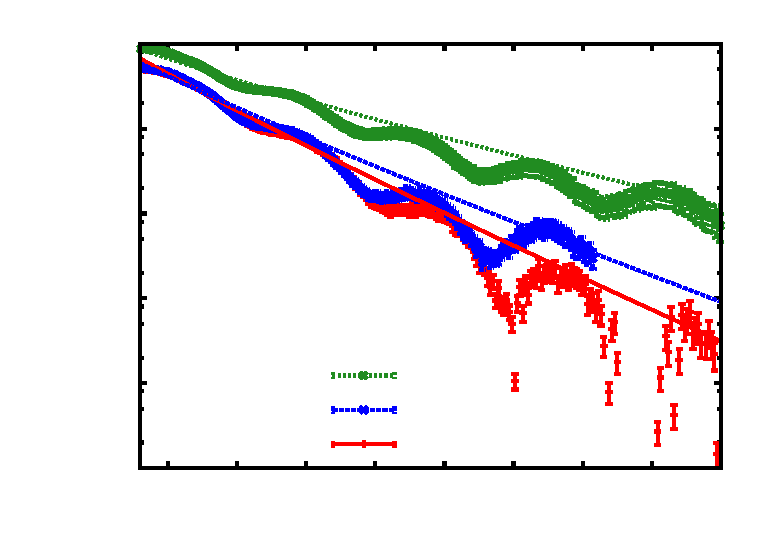
\includegraphics{fit_G6}}%
    \gplfronttext
  \end{picture}%
\endgroup
\end{Large}}
	\column{0.5\textwidth}\centering
	Dynamical correlation\\
	\resizebox{\columnwidth}{!}{\begin{Large}% GNUPLOT: LaTeX picture with Postscript
\begingroup
  \makeatletter
  \providecommand\color[2][]{%
    \GenericError{(gnuplot) \space\space\space\@spaces}{%
      Package color not loaded in conjunction with
      terminal option `colourtext'%
    }{See the gnuplot documentation for explanation.%
    }{Either use 'blacktext' in gnuplot or load the package
      color.sty in LaTeX.}%
    \renewcommand\color[2][]{}%
  }%
  \providecommand\includegraphics[2][]{%
    \GenericError{(gnuplot) \space\space\space\@spaces}{%
      Package graphicx or graphics not loaded%
    }{See the gnuplot documentation for explanation.%
    }{The gnuplot epslatex terminal needs graphicx.sty or graphics.sty.}%
    \renewcommand\includegraphics[2][]{}%
  }%
  \providecommand\rotatebox[2]{#2}%
  \@ifundefined{ifGPcolor}{%
    \newif\ifGPcolor
    \GPcolortrue
  }{}%
  \@ifundefined{ifGPblacktext}{%
    \newif\ifGPblacktext
    \GPblacktexttrue
  }{}%
  % define a \g@addto@macro without @ in the name:
  \let\gplgaddtomacro\g@addto@macro
  % define empty templates for all commands taking text:
  \gdef\gplbacktext{}%
  \gdef\gplfronttext{}%
  \makeatother
  \ifGPblacktext
    % no textcolor at all
    \def\colorrgb#1{}%
    \def\colorgray#1{}%
  \else
    % gray or color?
    \ifGPcolor
      \def\colorrgb#1{\color[rgb]{#1}}%
      \def\colorgray#1{\color[gray]{#1}}%
      \expandafter\def\csname LTw\endcsname{\color{white}}%
      \expandafter\def\csname LTb\endcsname{\color{black}}%
      \expandafter\def\csname LTa\endcsname{\color{black}}%
      \expandafter\def\csname LT0\endcsname{\color[rgb]{1,0,0}}%
      \expandafter\def\csname LT1\endcsname{\color[rgb]{0,1,0}}%
      \expandafter\def\csname LT2\endcsname{\color[rgb]{0,0,1}}%
      \expandafter\def\csname LT3\endcsname{\color[rgb]{1,0,1}}%
      \expandafter\def\csname LT4\endcsname{\color[rgb]{0,1,1}}%
      \expandafter\def\csname LT5\endcsname{\color[rgb]{1,1,0}}%
      \expandafter\def\csname LT6\endcsname{\color[rgb]{0,0,0}}%
      \expandafter\def\csname LT7\endcsname{\color[rgb]{1,0.3,0}}%
      \expandafter\def\csname LT8\endcsname{\color[rgb]{0.5,0.5,0.5}}%
    \else
      % gray
      \def\colorrgb#1{\color{black}}%
      \def\colorgray#1{\color[gray]{#1}}%
      \expandafter\def\csname LTw\endcsname{\color{white}}%
      \expandafter\def\csname LTb\endcsname{\color{black}}%
      \expandafter\def\csname LTa\endcsname{\color{black}}%
      \expandafter\def\csname LT0\endcsname{\color{black}}%
      \expandafter\def\csname LT1\endcsname{\color{black}}%
      \expandafter\def\csname LT2\endcsname{\color{black}}%
      \expandafter\def\csname LT3\endcsname{\color{black}}%
      \expandafter\def\csname LT4\endcsname{\color{black}}%
      \expandafter\def\csname LT5\endcsname{\color{black}}%
      \expandafter\def\csname LT6\endcsname{\color{black}}%
      \expandafter\def\csname LT7\endcsname{\color{black}}%
      \expandafter\def\csname LT8\endcsname{\color{black}}%
    \fi
  \fi
  \setlength{\unitlength}{0.0500bp}%
  \begin{picture}(7200.00,5040.00)%
    \gplgaddtomacro\gplbacktext{%
      \csname LTb\endcsname%
      \put(1056,704){\makebox(0,0)[r]{\strut{}$10^{-4}$}}%
      \put(1056,1938){\makebox(0,0)[r]{\strut{}$10^{-3}$}}%
      \put(1056,3171){\makebox(0,0)[r]{\strut{}$10^{-2}$}}%
      \put(1056,4405){\makebox(0,0)[r]{\strut{}$10^{-1}$}}%
      \put(1368,484){\makebox(0,0){\strut{}$2$}}%
      \put(2266,484){\makebox(0,0){\strut{}$3$}}%
      \put(3165,484){\makebox(0,0){\strut{}$4$}}%
      \put(4064,484){\makebox(0,0){\strut{}$5$}}%
      \put(4963,484){\makebox(0,0){\strut{}$6$}}%
      \put(5861,484){\makebox(0,0){\strut{}$7$}}%
      \put(6760,484){\makebox(0,0){\strut{}$8$}}%
      \put(286,2740){\rotatebox{-270}{\makebox(0,0){\strut{}$\mathcal{G}_u(r,t^{dh})/\Delta r^2(t^{dh})$}}}%
      \put(6979,2740){\rotatebox{-270}{\makebox(0,0){\strut{}}}}%
      \put(3974,154){\makebox(0,0){\strut{}$r/\sigma$}}%
      \put(3974,4666){\makebox(0,0){\strut{}}}%
      \put(3974,4665){\makebox(0,0){\strut{}}}%
      \put(-264,110){\makebox(0,0)[l]{\strut{}}}%
    }%
    \gplgaddtomacro\gplfronttext{%
      \csname LTb\endcsname%
      \put(2904,932){\makebox(0,0)[r]{\strut{}$\phi=0.497$}}%
      \csname LTb\endcsname%
      \put(2904,1262){\makebox(0,0)[r]{\strut{}$\phi=0.555$}}%
      \csname LTb\endcsname%
      \put(2904,1592){\makebox(0,0)[r]{\strut{}$\phi=0.576$}}%
    }%
    \gplbacktext
    \put(0,0){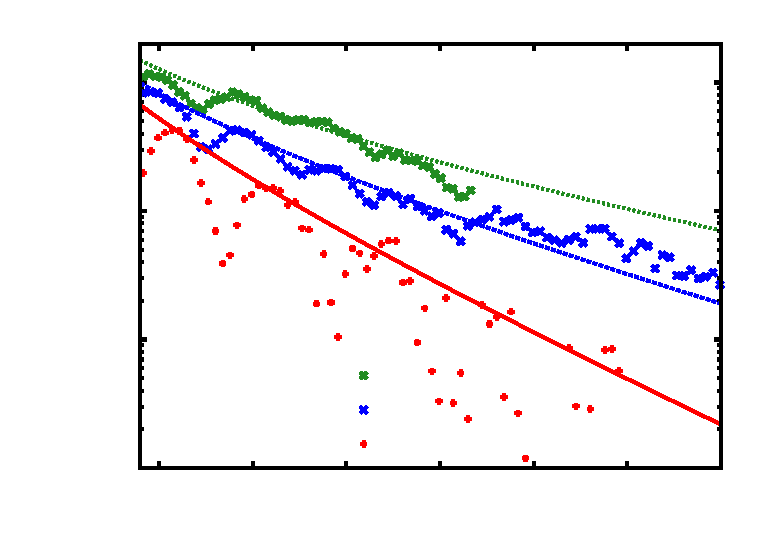
\includegraphics{fit_gu}}%
    \gplfronttext
  \end{picture}%
\endgroup
\end{Large}}	
	\end{columns}
	\begin{itemize}
		\item Ornstein-Zernike fit for both
		\begin{itemize}
			\item Indication of criticality
		\end{itemize}
		\item No icosahedra here, only crystal-like order
	\end{itemize}
\end{frame}

\begin{frame}{Diverging correlation lengths}
	\begin{textblock*}{0.6\textwidth}(10mm,92mm)
		\simplephasediagram{}
	\end{textblock*}
	\begin{columns}
	\column{0.5\textwidth}\centering
	\resizebox{\columnwidth}{!}{\begin{Large}\input{fit_xi.tex}\end{Large}}
	\column{0.5\textwidth}\centering
	Power-law fit
	\[ \xi(\phi) \propto \xi_0 \left( \frac{\phi_0 - \phi}{\phi} \right)^{-\frac{2}{3}} \]
	\end{columns}
	\begin{itemize}
		\item $\phi_0$ comes from the divergence of $\tau_\alpha$
		\item $\xi_0$ is the only adjustable parameter
		\item Exponent compatible with the Ising universality class
	\end{itemize}
	The divergence of the dynamics is linked to the crystal-like order
\end{frame}

\subsection{Structures and mobility}

\begin{frame}{Where are the fast particles ?}
	\begin{textblock*}{0.6\textwidth}(10mm,92mm)
		\simplephasediagram{}
	\end{textblock*}
	\begin{columns}
	\column{0.6\textwidth}
	\resizebox{\columnwidth}{!}{% GNUPLOT: LaTeX picture with Postscript
\begingroup
  \makeatletter
  \providecommand\color[2][]{%
    \GenericError{(gnuplot) \space\space\space\@spaces}{%
      Package color not loaded in conjunction with
      terminal option `colourtext'%
    }{See the gnuplot documentation for explanation.%
    }{Either use 'blacktext' in gnuplot or load the package
      color.sty in LaTeX.}%
    \renewcommand\color[2][]{}%
  }%
  \providecommand\includegraphics[2][]{%
    \GenericError{(gnuplot) \space\space\space\@spaces}{%
      Package graphicx or graphics not loaded%
    }{See the gnuplot documentation for explanation.%
    }{The gnuplot epslatex terminal needs graphicx.sty or graphics.sty.}%
    \renewcommand\includegraphics[2][]{}%
  }%
  \providecommand\rotatebox[2]{#2}%
  \@ifundefined{ifGPcolor}{%
    \newif\ifGPcolor
    \GPcolortrue
  }{}%
  \@ifundefined{ifGPblacktext}{%
    \newif\ifGPblacktext
    \GPblacktexttrue
  }{}%
  % define a \g@addto@macro without @ in the name:
  \let\gplgaddtomacro\g@addto@macro
  % define empty templates for all commands taking text:
  \gdef\gplbacktext{}%
  \gdef\gplfronttext{}%
  \makeatother
  \ifGPblacktext
    % no textcolor at all
    \def\colorrgb#1{}%
    \def\colorgray#1{}%
  \else
    % gray or color?
    \ifGPcolor
      \def\colorrgb#1{\color[rgb]{#1}}%
      \def\colorgray#1{\color[gray]{#1}}%
      \expandafter\def\csname LTw\endcsname{\color{white}}%
      \expandafter\def\csname LTb\endcsname{\color{black}}%
      \expandafter\def\csname LTa\endcsname{\color{black}}%
      \expandafter\def\csname LT0\endcsname{\color[rgb]{1,0,0}}%
      \expandafter\def\csname LT1\endcsname{\color[rgb]{0,1,0}}%
      \expandafter\def\csname LT2\endcsname{\color[rgb]{0,0,1}}%
      \expandafter\def\csname LT3\endcsname{\color[rgb]{1,0,1}}%
      \expandafter\def\csname LT4\endcsname{\color[rgb]{0,1,1}}%
      \expandafter\def\csname LT5\endcsname{\color[rgb]{1,1,0}}%
      \expandafter\def\csname LT6\endcsname{\color[rgb]{0,0,0}}%
      \expandafter\def\csname LT7\endcsname{\color[rgb]{1,0.3,0}}%
      \expandafter\def\csname LT8\endcsname{\color[rgb]{0.5,0.5,0.5}}%
    \else
      % gray
      \def\colorrgb#1{\color{black}}%
      \def\colorgray#1{\color[gray]{#1}}%
      \expandafter\def\csname LTw\endcsname{\color{white}}%
      \expandafter\def\csname LTb\endcsname{\color{black}}%
      \expandafter\def\csname LTa\endcsname{\color{black}}%
      \expandafter\def\csname LT0\endcsname{\color{black}}%
      \expandafter\def\csname LT1\endcsname{\color{black}}%
      \expandafter\def\csname LT2\endcsname{\color{black}}%
      \expandafter\def\csname LT3\endcsname{\color{black}}%
      \expandafter\def\csname LT4\endcsname{\color{black}}%
      \expandafter\def\csname LT5\endcsname{\color{black}}%
      \expandafter\def\csname LT6\endcsname{\color{black}}%
      \expandafter\def\csname LT7\endcsname{\color{black}}%
      \expandafter\def\csname LT8\endcsname{\color{black}}%
    \fi
  \fi
  \setlength{\unitlength}{0.0500bp}%
  \begin{picture}(7200.00,5040.00)%
    \gplgaddtomacro\gplbacktext{%
      \csname LTb\endcsname%
      \put(1254,699){\makebox(0,0)[r]{\strut{}$0.00$}}%
      \put(1254,1718){\makebox(0,0)[r]{\strut{}$0.05$}}%
      \put(1254,2738){\makebox(0,0)[r]{\strut{}$0.10$}}%
      \put(1254,3757){\makebox(0,0)[r]{\strut{}$0.15$}}%
      \put(1254,4776){\makebox(0,0)[r]{\strut{}$0.20$}}%
      \put(2228,484){\makebox(0,0){\strut{}$0.51$}}%
      \put(3523,484){\makebox(0,0){\strut{}$0.53$}}%
      \put(4818,484){\makebox(0,0){\strut{}$0.55$}}%
      \put(6113,484){\makebox(0,0){\strut{}$0.57$}}%
      \put(484,2740){\rotatebox{90}{\makebox(0,0){\strut{}Proportion of the 10\% fastest particles}}}%
      \put(6979,2740){\rotatebox{90}{\makebox(0,0){\strut{}}}}%
      \put(4073,154){\makebox(0,0){\strut{}$\phi$}}%
      \put(4073,4666){\makebox(0,0){\strut{}}}%
      \put(4073,4665){\makebox(0,0){\strut{}}}%
      \put(330,110){\makebox(0,0)[l]{\strut{}}}%
    }%
    \gplgaddtomacro\gplfronttext{%
      \csname LTb\endcsname%
      \put(4422,4556){\makebox(0,0)[r]{\strut{}in Crystal-like}}%
      \csname LTb\endcsname%
      \put(4422,4241){\makebox(0,0)[r]{\strut{}in Icosahedron}}%
      \csname LTb\endcsname%
      \put(4422,3926){\makebox(0,0)[r]{\strut{}in perfect Icosahedron}}%
    }%
    \gplbacktext
    \put(0,0){\includegraphics{proportions_phi}}%
    \gplfronttext
  \end{picture}%
\endgroup
}
	\column{0.4\textwidth}
	\[ \frac{\#(\text{fast}\cap\text{icosahedron})}{\#(\text{icosahedron})} \]
	\end{columns}
	\begin{itemize}
		\item Crystal-like particles are slow
		\item Perfect icosahedra are slow
		\item Imperfect icosahedra are as the bulk or even faster
	\end{itemize}
\end{frame}

\begin{frame}{Bond order dynamic propensity}
	\tikzstyle{na} = [baseline=-.5ex, remember picture]
	\begin{columns}
	\column{0.5\textwidth}
	\centering{\resizebox{\columnwidth}{!}{\input{w6Q6quarter.pdf_tex}}}
	\column{0.5\textwidth}
	\begin{itemize}
		%Label some of the idems by invisible nodes
		\item\colorbox{red!20}{Mean square displacement}
		\item\colorbox{green!20}{Same initial structure} (bond order)
		\item\colorbox{blue!20}{Ensemble average}
		\item Select only the influence of the bond order
	\end{itemize}
	\end{columns}
	\begin{equation*}
	%labelling parts of the equation with colors. Makes the equation code impossible to read
	\mathcal{P}r(w_6, Q_6, t) \equiv \frac{
		\colorbox{blue!20}{$\sum\limits_{t_0=0}^{t_{max}-t} \sum\limits_i^N$}
		{
			\colorbox{red!20}{$\left\|\vec{r_i}(t_0+t)-\vec{r_i}(t_0)\right\|^2$}
            \colorbox{green!20}{$\delta(w_6^i-w_6) \delta(Q_6^i-Q_6)$}
		}
	}{
		\sum\limits_{t_0=0}^{t_{max}-t} \sum\limits_i{ \delta(w_6^i-w_6) \delta(Q_6^i-Q_6)}
	}
	\end{equation*}
\end{frame}

\begin{frame}{Bond order dynamic propensity}
	\begin{textblock*}{0.6\textwidth}(10mm,92mm)
		\simplephasediagram{}
	\end{textblock*}
	\begin{columns}
	\column{0.68\textwidth}
	\resizebox{1.1\columnwidth}{!}{\input{msd_w6Q6quarter.pdf_tex}}
	\column{0.32\textwidth}
	\begin{itemize}
		\item Crystal-like particles are \alert{very slow}
		\item Perfect icosahedra are slow
		\item Imperfect icosahedra are as the bulk
	\end{itemize}
	\end{columns}
\end{frame}

\begin{frame}{Slow structures}
	\begin{textblock*}{0.6\textwidth}(10mm,92mm)
		\simplephasediagram{%
		\node at (0.568,0) [xp marker, fill=green!50!black] {};
		}
	\end{textblock*}
	\begin{columns}[T]
	\column{0.6\textwidth}
	\only<all:1>{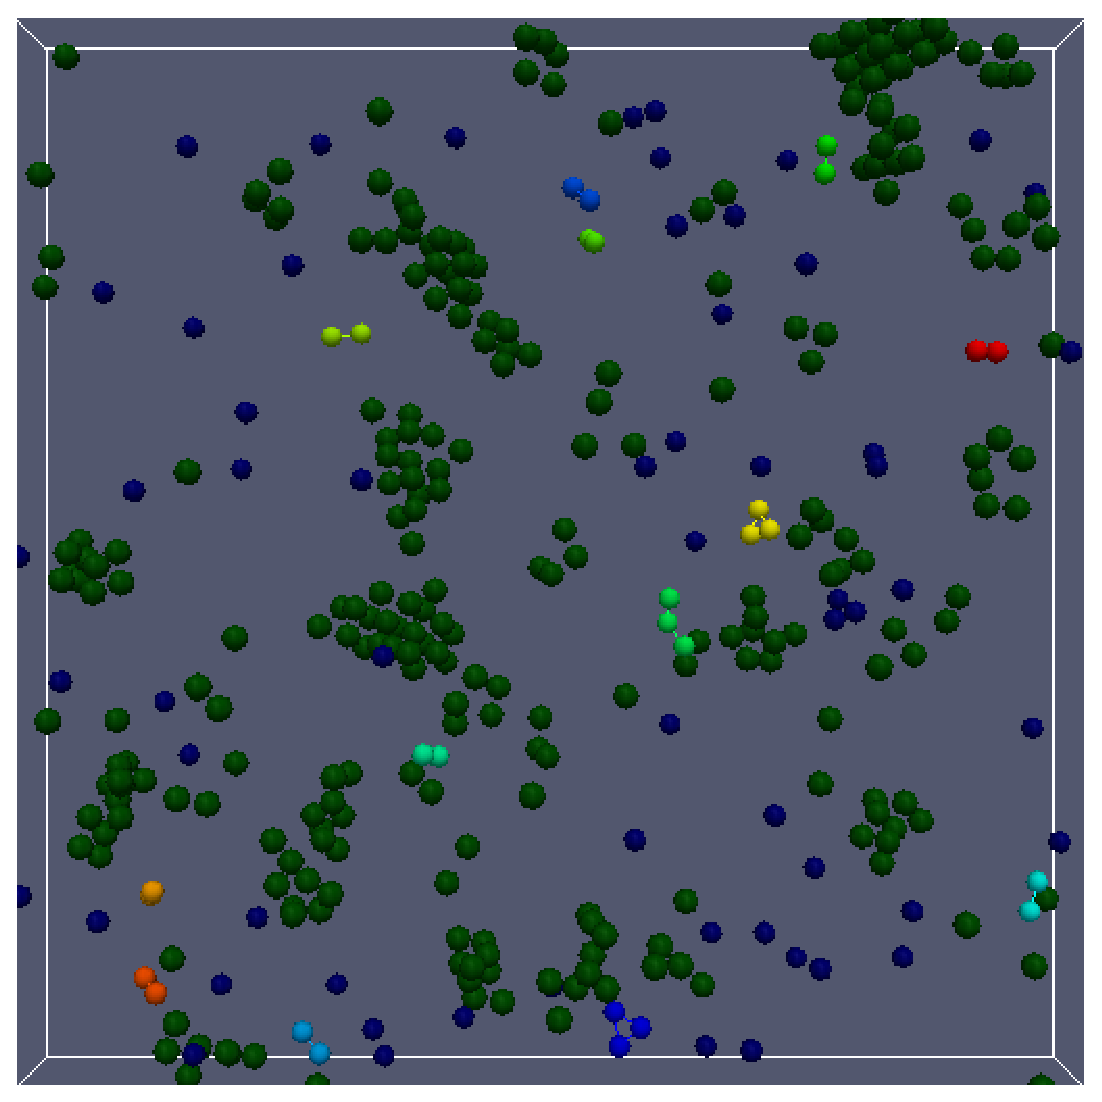
\includegraphics[width=\columnwidth]{stable_only_ico_go1}}%
	\only<all:2>{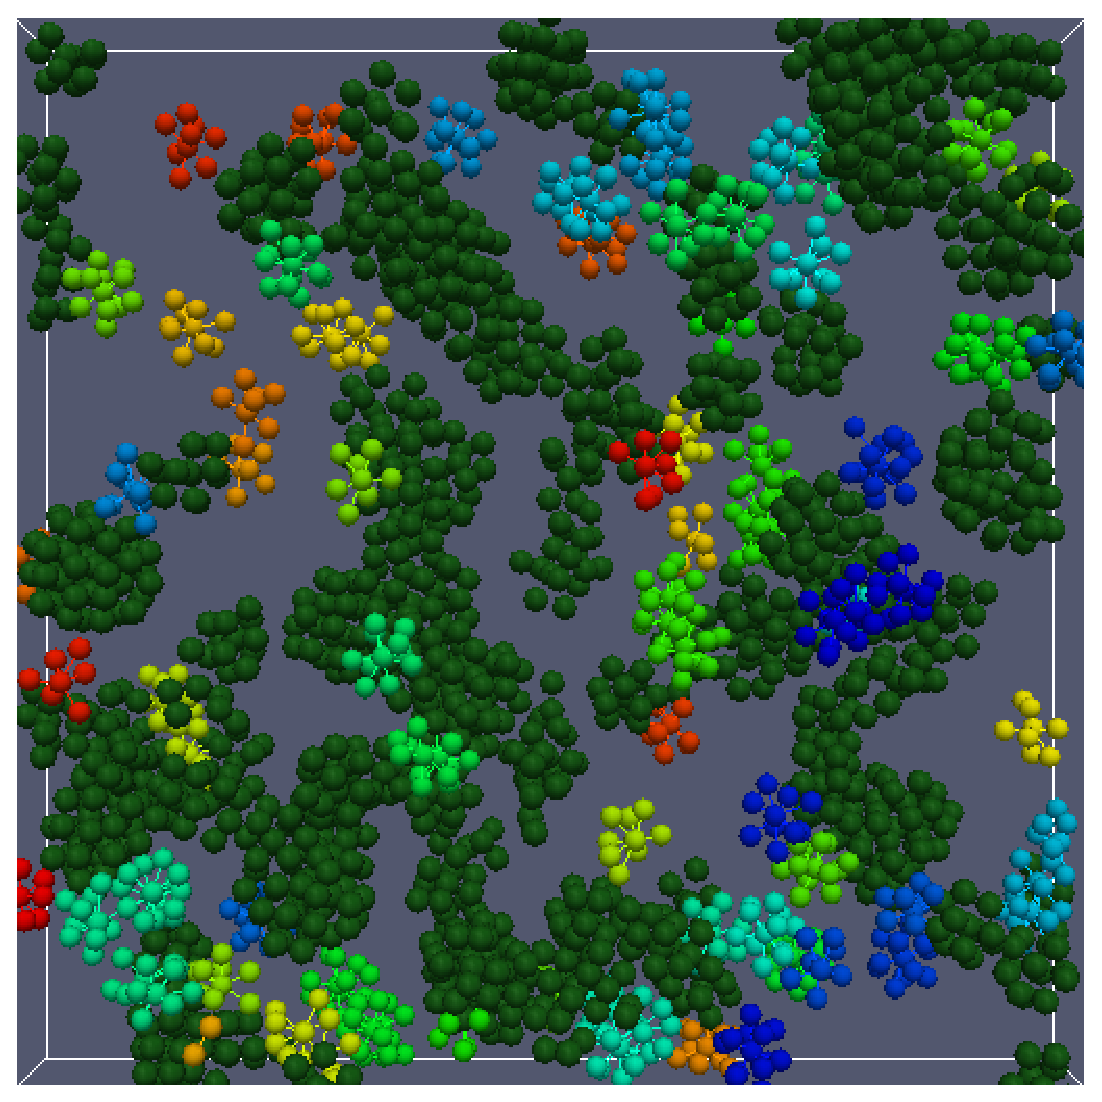
\includegraphics[width=\columnwidth]{mrco_stable_ico_ngb_go1}}%
	\[ \phi=0.568 \]
	\column{0.4\textwidth}
	\begin{block}{\only<all:1>{Central particle}\only<all:2>{Centre and neighbours}}
	\begin{itemize}
		\item Crystal-like \tikz\shade[ball color=green!33!black] (0,0) circle (0.5em);
		\item Perfect Icosahedra\only<all:1>{
		\begin{itemize}
			\item isolated \tikz\shade[ball color=blue!50!black] (0,0) circle (0.5em);
			\item connected} 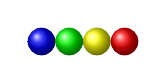
\begin{tikzpicture}
				\shade[ball color=blue] (0,0) circle (0.5em);
				\shade[ball color=green] +(1em,0) circle (0.5em);
				\shade[ball color=yellow] +(2em,0) circle (0.5em);
				\shade[ball color=red] +(3em,0) circle (0.5em);
				\end{tikzpicture}%
		\only<all:1>{\end{itemize}}%
	\end{itemize}
	\end{block}
	Near the glass transition
	\begin{itemize}
		\item Slow structures are mainly crystal-like
		\item Perfect icosahedra do not reach medium range size
	\end{itemize}
	\end{columns}
\end{frame}

\section*{Conclusion}

\begin{frame}{Summary}
	\begin{itemize}
		\item Crystal-like bond order
		\begin{itemize}
			\item The divergence of the dynamics toward the ideal glass transition is 
			\begin{itemize}
				\item linked to the crystal-like bond order
				\item of a critical nature
			\end{itemize}
			\item The crystal-like bond order is responsible for the dynamical arrest
		\end{itemize}
		
		\item Icosahedral order 
		\begin{itemize}
			\item exists even without attraction
			\item form a low dimensional \alert{unstable} network
			\item may have an important role in
			\begin{itemize}
				\item the avoidance of crystallisation
				\item the fragility of the glass former
			\end{itemize}
		\end{itemize}
		\item Few icosahedra are stable
		\begin{itemize}
			\item counter-intuitive free volume stabilisation
			\item are not reaching medium range size
			\item have no influence on the dynamical arrest
		\end{itemize}
	\end{itemize}
\end{frame}

\begin{frame}{Conclusion}
	\begin{itemize}
		\item A static correlation length is linked to the glass transition
		\item The important structure is
		\begin{itemize}
			\item the one linked to the avoided first order transition
			\item not an unreachable ground state
		\end{itemize}
		\item Other type of order can appear locally as a source of frustration
		\item Icosahedral order can be present with negligible effect on the dynamics
	\end{itemize}
\end{frame}